\section{Torque Converter Attention}


通常、注意はフィルタ、重み、選択、抑制として語られる。

どの情報を通すのか。どの対象に焦点を当てるのか。どの表象を強め、どの表象を弱めるのか。

これらの記述は、静的な処理モデルでは有効である。

しかし本稿で扱う意識モデルにおいて、注意の中心問題は選択ではない。

中心にあるのは、異なる速度で走る処理を、同一速度へ潰さずに接続することである。

高速な予測流と低速な記憶流は、そのままでは直接接続できない。

高速層は変化が速く、揮発的であり、現在に先行する。

低速層は変化が遅く、沈殿的であり、過去を保持する。

両者を剛体的に結合すれば、速度差は失われる。

逆に、完全に分離すれば、ログ参照は成立しない。

したがって必要なのは、速度差を消さず、しかし破綻もさせない中間機構である。

本稿では、この機構をトルクコンバータ・アテンションと呼ぶ。

\subsection{Why Filter, Gate, Weight, and Switch Are Insufficient}

既存の注意モデルで頻繁に用いられる語には、それぞれ限界がある。

filter は、通すか通さないかを表すが、速度差そのものを扱えない。

gate は、入口と出口を示すが、内部で生じる滑りや遅延を消してしまう。

weight は、重要度を数値化できるが、処理速度の差を含まない。

switch は、状態の切り替えを表すが、連続的な変換や部分的な結合を表現しにくい。

これらはいずれも、選択や強度を扱う語である。

しかし、本稿で必要なのは、選択の語ではなく、時間変換の語である。

注意とは、何を選ぶか以前に、異なる時間スケールの処理がどのように接続されるかという問題である。

\subsection{Torque Converter as Structural Analogy}

トルクコンバータは、異なる角速度をもつ二つの回転系を剛体的に固定せず、流体的な滑りを許しながら力を伝達する装置である。

ここで重要なのは、速度差が欠陥ではないという点である。

トルクコンバータは、速度差を消してから力を伝えるのではない。

速度差を保持したまま、その差を破綻しない形で伝達可能にする。

この構造は、本稿における高速層と低速層の関係に対応する。

高速層と低速層のあいだには、速度差 $\Delta v$ がある。

\begin{equation}
\Delta v = v_f - v_s
\end{equation}

この速度差がなければ、参照のための境界は開かれない。

しかし速度差が大きすぎれば、参照は断片化する。

したがって必要なのは、差を消す機構ではなく、差を変換する機構である。

これが、トルクコンバータ・アテンションである。

\subsection{Effective Torque}

速度差が変換負荷として現れる量を、有効トルク様量 $\mathcal{T}$ と表す。

\begin{equation}
\mathcal{T}
=
\kappa
\frac{\Delta v}{\mu}
\end{equation}

ここで、$\kappa$ はスケール係数、$\mu$ は結合粘性である。

$\mu$ は、速度スケール間の滑りや結合の粘りを表す。

$\mu$ が小さすぎれば、二つの層は過剰に密着し、速度差が潰れやすくなる。

$\mu$ が大きすぎれば、二つの層は滑りすぎ、参照は不安定化する。

したがって、$\mathcal{T}$ は単なる力の大きさではない。

それは、速度差が結合粘性を介してどれだけ変換負荷として現れるかを表す構造的指標である。

ここで注意すべきなのは、$\mathcal{T}$ を心理的意志や主体性の量として読まないことである。

$\mathcal{T}$ は「どれだけ意識が強いか」を表す量ではない。

それは、異なる速度で走る処理が、ログ参照可能な関係へ変換されるための負荷である。

\cref{fig:tca-ja} は、TCA が速度差を消さずに変換する構造を示している。

\begin{figure}[H]
\centering
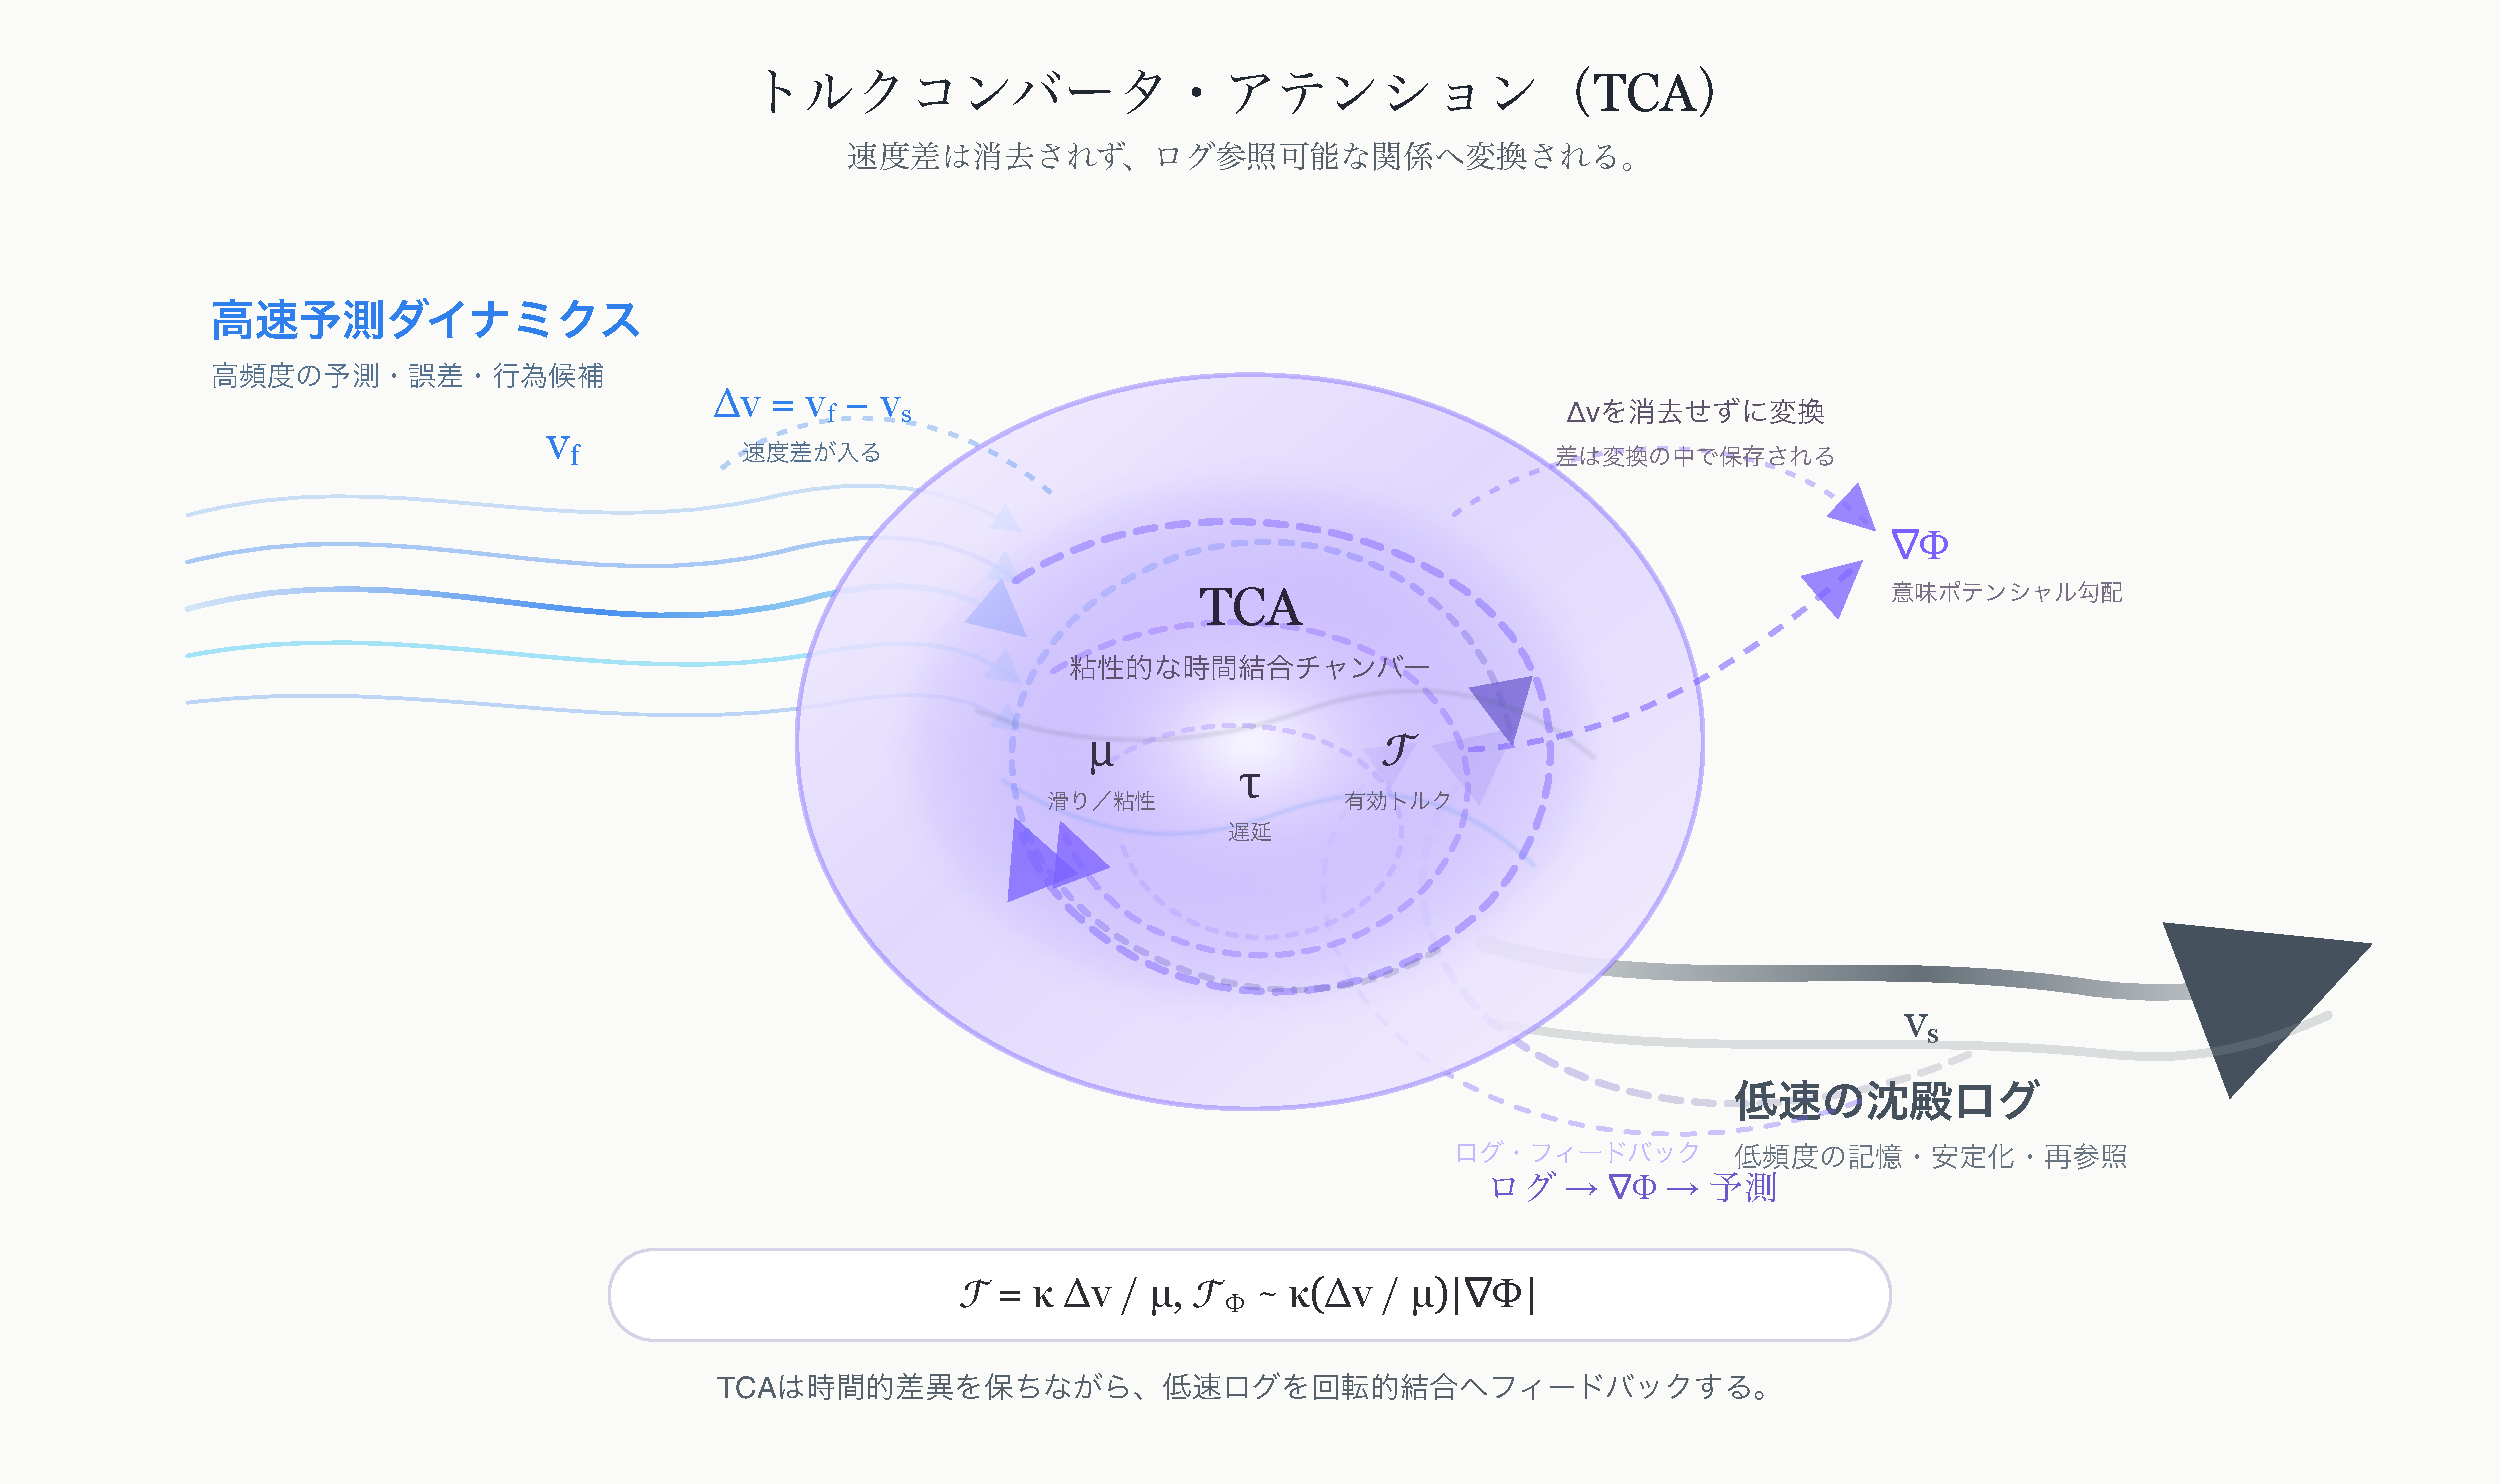
\includegraphics[width=0.92\linewidth]{figures_ja/figure2_tca_jp.pdf}
\caption{
Torque Converter Attention（TCA）。
TCA は時間的差異を保持したまま、それをログ参照可能な関係へ変換する。
高速な予測ダイナミクス、低速な沈殿ログ、結合粘性、遅延、有効トルク様量は、速度差を消去せずに結合される。
}
\label{fig:tca-ja}
\end{figure}

局所的に見れば、あるログまたは概念地形要素 $i$ への注意重み $A_i$ は、そのログの情報質量、または沈殿度 $m_i$ と、局所的な有効トルク様量 $\mathcal{T}_i$ の積として表される。

\begin{equation}
A_i \propto m_i \cdot \mathcal{T}_i
\end{equation}

ここで $\mathcal{T}_i$ は、心理的な意志の量ではなく、高速層と低速層の速度差から生じる局所的な変換負荷である。

\begin{equation}
\mathcal{T}_i \propto \Delta v_i
\end{equation}

したがって、最小近似では次のように書ける。

\begin{equation}
A_i \propto m_i \cdot \Delta v_i
\end{equation}

この式は、注意を単なる選択ではなく、保存されたログの質量と現在の速度差トルクの積として捉えるためのものである。

ここで、SSO の速度差、IFGT の情報ポテンシャル、Conceptual Topography における概念地形要素の沈殿度が接続される。

\subsection{Attention as Temporal Transformation}

この立場から見ると、Attention は選択機構ではなく、時間変換機構である。

Attention は、速い処理を遅い処理へそのままコピーするものではない。

また、遅い処理が速い処理を上から制御するものでもない。

Attention は、高速層で生じた予測、期待、誤差、反応を、低速層が参照可能な時間幅へ変換する。

この変換には遅延 $\tau$ が伴う。

\begin{equation}
\tau \propto \frac{\Delta v}{\mu}
\end{equation}

この遅延は単なる処理遅れではない。

それは、現在処理が過去ログへ沈殿し、再参照可能になるための時間的厚みである。

したがって、Attention は「どこを見るか」ではなく、「どの速度差を、どの時間幅で、どの程度滑らせながら通過させるか」を決める構造である。

この意味で、Attention は心理語ではなく、時間制御語である。

\begin{quote}
\textbf{CT との対応（Conceptual Topography §4.2）：} 概念地形論では、言語トークン $\ell_{i}$ が $\nabla\Phi$ に局所結合し、繰り返し使用によってポテンシャル井戸を深化させる。この結合項
\[
\lambda \sum_i \ell_{i} \cdot \nabla\Phi
\]
は、本稿のTCAが行う「速度差を意味勾配に沿って変換する」操作と対応している。TCAは時間軸上の変換機構であり、CT のトークン結合は空間軸上の変換機構である。両者は同一の変換構造の異なる断面として読める。
\end{quote}

\subsection{From Attention to Ego}

本稿では、このトルクコンバータ・アテンションが、体験上は自我として感じられる位置に対応すると考える。

ただし、ここでいう自我は主体ではない。

自我は判断者でも、司令塔でも、意思決定者でもない。

自我とは、高速層と低速層の速度差が集中し、変換される力学的位置である。

人間はこの変換点を、自分が考えている場所、自分が選んでいる場所、自分が意識している場所として経験しやすい。

しかし、それは自我が行動の原因であることを意味しない。

むしろ、自我とは、行動準備、記憶沈殿、ログ参照が交差する点である。

このため、自我は幻想ではない。

それは明確な機能を持つ。

しかし同時に、自我は主体でもない。

それは、二重可塑性と時間非対称性が成立したときに要請される変換点である。

\subsection{Relation to Log Referencing}

トルクコンバータ・アテンションが重要なのは、それがログ参照を可能にするからである。

高速層で生じた処理は、そのままでは消えていく。

低速層に沈殿したログは、そのままでは現在に接続されない。

両者の間にトルクコンバータ・アテンションが働くことで、現在処理と過去ログの間に参照関係が開かれる。

このとき、高速層の処理は低速層に完全に吸収されるわけではない。

低速層のログも、高速層を完全に支配するわけではない。

両者は、速度差を保持したまま結合する。

この非閉包的な結合が、ログ参照状態としての意識の前提になる。

\subsection{Bridge to IFGT and VED}

ここまでの議論では、トルクコンバータ・アテンションを速度差と結合粘性の問題として定義した。

しかし、意識状態において、どのログが参照されやすいかは速度差だけでは決まらない。

ログ参照は、意味勾配によって方向づけられる。

そのため、次節では情報密度 $I$、情報流 $J_I$、局所的なログ参照流 $J_{\log}$、情報ポテンシャル $\Phi$ を導入し、このトルク様量を IFGT/VED の構造へ写像する。

そこで、有効トルク様量 $\mathcal{T}$ は、意味勾配を含む拡張量 $\mathcal{T}_{\Phi}$ へと拡張される。

\begin{equation}
\mathcal{T}_{\Phi}
\sim
\kappa
\frac{\Delta v}{\mu}
|\nabla \Phi|
\end{equation}

この式は、意識を生成する式ではない。

それは、速度差、結合粘性、意味勾配が同時に成立したとき、ログ参照がどの方向へ開かれやすいかを示す構造的指標である。

したがって、トルクコンバータ・アテンションは、本稿において単なる比喩ではない。

それは、速度差を非閉包のまま保持する VED 的機構であり、意味勾配に沿ってログ参照を方向づける IFGT 的機構でもある。
